{\sihao \color{MsBlue} \kaishu 2. {\bfseries 项目的研究内容、研究目标,以及拟解决的关键科学问题}(此部分为重点阐述内容);}

\subsubsection{\bfseries 2.1 研究内容:}
% 未完成

\noindent{\bfseries 研究内容 1:}

\noindent{\bfseries 研究内容 2:}

\noindent{\bfseries 研究内容 3:}

见\cref{fig:sample-tikz}。

\begin{figure}[!htp]
\centering
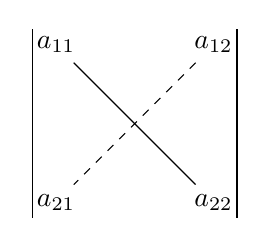
\begin{tikzpicture}
\node at (0,2) (a11) {$a_{11}$};
\node at (2,2) (a12) {$a_{12}$};
\node at (0,0) (a21) {$a_{21}$};
\node at (2,0) (a22) {$a_{22}$};
\draw (-0.3, 2.2) -- (-0.3, -0.2);
\draw (2.3, 2.2) -- (2.3, -0.2);
\draw (a11) -- (a22);
\draw[dashed] (a12) -- (a21);
\end{tikzpicture}
\caption{Tikz示例图}
\label{fig:sample-tikz}
\end{figure}


见\cref{fig:sample-fig}。

\begin{figure}[!htp]
\centering
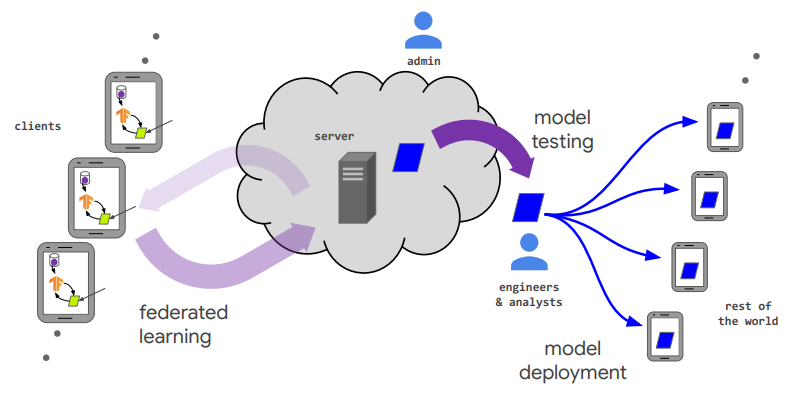
\includegraphics[width=0.75\textwidth]{figures/sample-fig.png}
\caption{示例图}
\label{fig:sample-fig}
\end{figure}


\subsubsection{\bfseries 2.2 研究目标:}
% 未完成

本项目针对待写。。。。


\subsubsection{\bfseries 2.3 关键问题:}
% 未完成

待写。。。。


\ifhandout
% do nothing
\else
\begin{center}
{\larger[2]\color{red} \ding{43}\ding{43} 研究内容部分共计 \wordcount 字 \reflectbox{\ding{43}\ding{43}}}
\end{center}
\fi


\vskip 5mm
